\subsection{Método Global}

\begin{figure}[H]
    \centering
    \begin{subfigure}{0.6\textwidth}
        \centering\newlength{\figwidth}\setlength{\figwidth}{0.9\textwidth}
        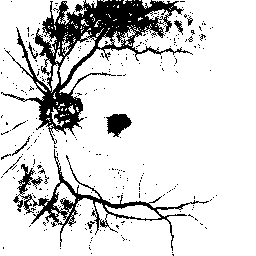
\includegraphics[width=0.6\figwidth]{global/retina.png}
        \caption{\texttt{retina.pgm} com $T = 128$. 15\% de pixels pretos.}
    \end{subfigure}\\[8pt]
    \metodo{wedge}{global/wedge100.png}{$T = 100$}{72}%
    \metodo{wedge}{global/wedge110.png}{$T = 110$}{49}

    \caption{Método Global.}
    \label{fig:global}
\end{figure}
